% !TeX program = xelatex
\documentclass[12pt,spanish,letterpaper,oneside]{article}
\PassOptionsToPackage{es-noshorthands}{babel}
\def\documenttitle{Prototipo Casero de Excavadora Hidráulica Articulada: Aplicación del Principio de Pascal en la Maquinaria Agrícola}
\def\documentsubtitle{Producto Integrador de Aprendizaje (PIA) --- Unidad de Aprendizaje: Física}
\def\documentsubject{Física (REF\#261013755808) --- 2.º Semestre}
\def\documentauthor{Diego de la Cruz Muñoz}
\def\coursename{Física}
\def\coursecode{REF\#261013755808}
\def\universityname{Universidad Autónoma de Nuevo León}
\def\universityfaculty{Facultad de Agronomía}
\def\universitydepartment{Licenciatura en Ingeniero Agrónomo}
\def\universitydepartmentimage{departamentos/logos-institucionales.pdf}
\def\universitydepartmentimagecfg{height=2.1cm}
\def\universitylocation{General Escobedo / Marín, Nuevo León, México}
\def\authortable{%
	\begin{Form}
	\begin{tabular}{@{}ll@{}}
		\textbf{Estudiante:} & Diego de la Cruz Muñoz\\[0.30cm]
		\textbf{Matrícula:} & 1977875\\[0.30cm]
		\textbf{Semestre y Grupo:} & 2.º Semestre --- Licenciatura en Ingeniero Agrónomo\\[0.30cm]
		\textbf{Docente Titular:} & Mtra. Elizabeth Garza Valverde\\[0.30cm]
		\textbf{Unidad de Aprendizaje:} & Física (Ponderación: 25 Puntos)\\[0.30cm]
		\textbf{Actividad Curricular:} & Producto Integrador de Aprendizaje (Actividad 4.1)\\[0.30cm]
		\textbf{Modalidad de Trabajo:} & Individual\\[0.30cm]
		\textbf{Fecha de Entrega en Plataforma:} & 13 de noviembre de 2026\\[0.45cm]
		\multicolumn{2}{l}{\universitylocation}
	\end{tabular}
	\end{Form}
}

\usepackage{fontspec}
\setmainfont{Arial}
\setsansfont{Arial}
% ==============================================================================
% ADAPTACIÓN INSTITUCIONAL - UANL (FACULTAD DE AGRONOMÍA) - FÍSICA
% AulaTeX / Licenciatura en Ingeniero Agrónomo
% ==============================================================================

\AddToHook{file/config.tex/after}[aulatex-fisica]{%
  \def\documentfontsize{12}
  \def\documentinterline{1.15}
  \def\documentparindent{0}
  \def\documentparskip{5}
  \def\fontdocument{custom}
  \def\fonttypewriter{custom}
  \def\stylecitereferences{custom}
  \def\portraitstyle{style1}
  \def\hfstyle{style1}
  \def\hfwidthwrap{false}
  \def\hfwidthtitle{0.60}
  \def\hfwidthcourse{0.38}
  \def\predocpageromannumber{false}
  \def\pagemarginleft{2.5}
  \def\pagemarginright{2.5}
  \def\pagemargintop{2.5}
  \def\pagemarginbottom{2.5}
  \def\firstpagemargintop{3.8}
  \def\sectionfontsize{\large}
  \def\sectionspacingtop{8}
  \def\sectionspacingbottom{4}
  \def\ssectionfontsize{\normalsize}
  \def\ssectionspacingtop{6}
  \def\ssectionspacingbottom{3}
  \def\defaultimagefolder{UANL/assets-uanl/}
  \def\usepdfmetadata{false}
}

% Carga del núcleo oficial de AulaTeX
% Template:     Informe LaTeX
% Documento:    Núcleo del template
% Versión:      DEV
% Codificación: UTF-8
%
% Autor: Pablo Pizarro R.
%        pablo@ppizarror.com
%
% Manual template: [https://latex.ppizarror.com/informe]
% Licencia MIT:    [https://opensource.org/licenses/MIT]

% -----------------------------------------------------------------------------
% CONFIGURACIONES
% -----------------------------------------------------------------------------
% Definiciones previas
\input{src/defs}

% Ajustes usuario
\input{src/config}

% -----------------------------------------------------------------------------
% IMPORTACIÓN DE LIBRERÍAS
% -----------------------------------------------------------------------------
\input{src/env/imports}

% -----------------------------------------------------------------------------
% IMPORTACIÓN DE FUNCIONES Y ENTORNOS
% -----------------------------------------------------------------------------
\input{src/cmd/core}
\input{src/cmd/math}
\input{src/cmd/equation}
\input{src/cmd/image}
\input{src/cmd/title}
\input{src/cmd/other}
\input{src/cmd/column}
\input{src/env/environments}

% -----------------------------------------------------------------------------
% IMPORTACIÓN DE ESTILOS
% -----------------------------------------------------------------------------
\input{src/style/code}
\input{src/style/other}

% -----------------------------------------------------------------------------
% CONFIGURACIÓN INICIAL DEL DOCUMENTO
% -----------------------------------------------------------------------------
\input{src/cfg/init}

% -----------------------------------------------------------------------------
% PORTADA
% -----------------------------------------------------------------------------
\input{src/page/portrait}
\input{src/page/portrait_config}

% -----------------------------------------------------------------------------
% CONFIGURACIÓN DE PÁGINA Y ENCABEZADOS
% -----------------------------------------------------------------------------
\input{src/cfg/page}

% -----------------------------------------------------------------------------
% TABLA DE CONTENIDOS - ÍNDICE
% -----------------------------------------------------------------------------
\input{src/page/index}

% -----------------------------------------------------------------------------
% CONFIGURACIONES FINALES
% -----------------------------------------------------------------------------
\input{src/cfg/final}

\RemoveFromHook{file/config.tex/after}[aulatex-fisica]

% Rutas de búsqueda de imágenes
\graphicspath{%
  {./figuras-pia/}%
  {./}%
  {UANL/assets-uanl/}%
  {../../UANL/assets-uanl/}%
  {../../../UANL/assets-uanl/}%
}

% Paleta institucional UANL / Agronomía
\definecolor{uanlblue}{RGB}{0,55,108}
\definecolor{uanlgreen}{RGB}{27,94,32}
\definecolor{tableblue}{RGB}{233,240,247}
\def\portraittitlecolor{uanlblue}
\def\sectioncolor{uanlblue}
\def\ssectioncolor{uanlgreen}

% Control de composición anti-huecos y balance de flotantes
\hfuzz=0.5pt
\vfuzz=0.5pt
\renewcommand{\topfraction}{0.90}
\renewcommand{\bottomfraction}{0.85}
\renewcommand{\textfraction}{0.07}
\renewcommand{\floatpagefraction}{0.85}
\renewcommand{\dbltopfraction}{0.90}
\renewcommand{\dblfloatpagefraction}{0.85}
\setcounter{topnumber}{3}
\setcounter{bottomnumber}{2}
\setcounter{totalnumber}{4}
\widowpenalty=10000
\clubpenalty=10000
\raggedbottom

\RequirePackage{etoolbox}
\RequirePackage{placeins}
\RequirePackage{needspace}
\RequirePackage{array}
\RequirePackage{ragged2e}
\RequirePackage{tabularx}
\RequirePackage{booktabs}
\RequirePackage{adjustbox}
\RequirePackage{eso-pic}
\RequirePackage{tikz}

% Marca de agua institucional oficial de la Facultad de Agronomía UANL en Portada
\makeatletter
\providecommand{\careerwatermarkimage}{UANL/assets-uanl/logo-agronomia.png}
\providecommand{\institutionalWatermark}[2][0.08]{%
  \global\let\aulatexWatermarkApplied\relax
  \AddToShipoutPictureBG*{%
    \put(0,0){%
      \parbox[b][\paperheight]{\paperwidth}{%
        \vfill
        \centering
        \begin{tikzpicture}[remember picture,overlay]
          \node[opacity=#1,inner sep=0pt] at (current page.center) {%
            \includegraphics[width=0.56\paperwidth]{#2}%
          };
        \end{tikzpicture}%
        \vfill
      }%
    }%
  }%
}
\pretocmd{\templatePortrait}{%
  \@ifundefined{aulatexWatermarkApplied}{%
    \institutionalWatermark[0.08]{\careerwatermarkimage}%
  }{}%
}{}{}

% Regla contractual: Pie de página bilateral estrictamente unilineal sin saltos
\AtBeginDocument{%
  \def\hfwidthwrap{false}%
  \fancyfoot[L]{\small\textit{\adjustbox{max width=0.60\linewidth}{\documenttitlehf}}}%
  \fancyfoot[R]{\small\textit{\adjustbox{max width=0.38\linewidth}{\coursename}}}%
}
\makeatother

\usepackage{tabularx}
\usepackage{booktabs}
\usepackage{amsmath,amssymb}
\usepackage{siunitx}
\usepackage{float}
\usepackage{graphicx}
\usepackage{subcaption}
\usepackage{tcolorbox}
\usepackage{setspace}
\setstretch{1.15}
\usepackage[backend=biber,style=apa,sorting=nyt]{biblatex}
\definecolor{uanlblue}{RGB}{0,55,108}
\definecolor{tableblue}{RGB}{233,240,247}
\def\portraittitlecolor{uanlblue}
\def\sectioncolor{uanlblue}
\def\ssectioncolor{uanlblue}
\def\documenttitlehf{Física (2.º Semestre): Prototipo Casero de Excavadora Hidráulica}
\hypersetup{colorlinks=true,linkcolor=uanlblue,urlcolor=uanlblue,citecolor=uanlblue,pdfauthor={Diego de la Cruz Muñoz},pdftitle={Prototipo Casero de Excavadora Hidraulica Articulada - PIA Fisica UANL},pdfsubject={Producto Integrador de Aprendizaje - Fisica Agronomia UANL}}
\addbibresource{UANL/ingeniero-agronomo/fisica/fisica.bib}
\newcolumntype{Y}{>{\raggedright\arraybackslash}X}
\setlength{\emergencystretch}{2.5em}

\begin{document}
\hypersetup{pageanchor=false}
\begingroup
\fontsize{14}{17}\selectfont
\renewcommand{\Huge}{\fontsize{14}{17}\selectfont\bfseries}
\renewcommand{\large}{\fontsize{14}{17}\selectfont}
\templatePortrait
\clearpage
\endgroup
\hypersetup{pageanchor=true}
\templatePagecfg
\setlength{\tabcolsep}{8pt}
\renewcommand{\arraystretch}{1.15}
\section*{Resumen}
En este Producto Integrador de Aprendizaje (PIA) para la materia de Física, como estudiante de segundo semestre de la carrera de Ingeniero Agrónomo en la Universidad Autónoma de Nuevo León, presento el diseño, la construcción casera y las pruebas de funcionamiento de un prototipo de excavadora hidráulica articulada. El objetivo principal de este trabajo es demostrar de forma práctica y visual el \textbf{Principio de Pascal}, comprendiendo cómo la presión que aplicamos sobre un líquido encerrado en reposo se transmite con la misma intensidad hacia todas direcciones y permite multiplicar la fuerza para mover un brazo mecánico. 

Para elaborar el prototipo utilicé materiales accesibles y fáciles de conseguir en casa y en la ferretería: tiras de madera reciclada cortadas con las medidas indicadas en el plano técnico (\SI{10.5}{cm}, \SI{17.5}{cm}, \SI{26.0}{cm} y \SI{36.0}{cm}), ocho jeringas plásticas conectadas por pares mediante mangueras delgadas transparentes, cinchos de plástico y agua de la llave pintada con colorante vegetal para detectar cualquier fuga o burbuja de aire. El prototipo cuenta con cuatro movimientos independientes controlados desde un panel manual: giro de la base, elevación de la pluma, articulación del brazo y apertura/cierre de la cuchara excavadora. Durante las pruebas caseras, comprobé que el sistema hidráulico transmite el movimiento de manera inmediata y permite levantar pequeñas cargas de tierra y sustrato agrícola sin esfuerzo, comprobando la importancia que tiene la hidráulica en la maquinaria que utilizamos en el campo, como retroexcavadoras y tractores con pala frontal. Se incluye la justificación, la memoria de construcción con fotografías, los resultados esperados y obtenidos, y el enlace del video explicativo de \SI{6}{minutos} y \SI{45}{segundos} grabado para la presentación grupal.

\vspace{0.25cm}
\noindent\textbf{Palabras clave:} Principio de Pascal, presión en fluidos, excavadora hidráulica, prototipo casero, maquinaria agrícola, agronomía.

\section{Justificación del Tema Elegido}
Al cursar el segundo semestre de la carrera de Ingeniero Agrónomo en la Facultad de Agronomía de la UANL, nos damos cuenta de que muchas de las actividades agrícolas dependen directamente de la maquinaria pesada y de los implementos que se acoplan al tractor \parencite{ortiz2003}. Cuando visitamos los campos de cultivo o las parcelas experimentales en Marín y Escobedo, observamos tractores, retroexcavadoras y palas mecánicas trabajando en labores fundamentales como:
\begin{itemize}
    \item \textbf{Apertura y mantenimiento de zanjas de desagüe:} En los suelos arcillosos de Nuevo León, el agua de lluvia o de riego en exceso puede quedarse estancada. Si no se cuenta con zanjas adecuadas, las raíces de los cultivos se quedan sin oxígeno (anoxia radicular) y la planta se marchita o enferma.
    \item \textbf{Tendido de mangueras de riego por goteo:} Para proteger las tuberías y mangueras de riego del sol, del paso del tractor y de los roedores, es necesario excavar zanjas angostas y uniformes donde se colocan las líneas de agua y fertilizante.
    \item \textbf{Carga y volteo de composta y abonos orgánicos:} El movimiento de estiércol, esquilmos y tierra vegetal requiere palas que puedan levantar cargas pesadas sin que el operador tenga que hacer un esfuerzo físico extremo.
\end{itemize}

Todas estas máquinas pesadas tienen algo en común: se mueven gracias a cilindros hidráulicos por los que circula aceite a presión. Elegí este tema porque representa una oportunidad perfecta para conectar lo que estamos aprendiendo en la clase de Física con los problemas reales que resolveremos como futuros agrónomos. Construir un prototipo casero con jeringas y agua me permitió ver con mis propios ojos cómo unas simples mangueras llenas de líquido pueden levantar peso y mover piezas pesadas, aplicando exactamente las mismas leyes que hacen funcionar a una retroexcavadora de verdad \parencite{serway2018}.

\section{Marco Conceptual y Principio Físico Demostrado}
\subsection{¿Qué es la Presión en un Fluido?}
En física, la presión ($P$) se define de manera sencilla como la cantidad de fuerza perpendicular ($F$) que se ejerce sobre una superficie o área determinada ($A$) \parencite{tippens2011}:
\begin{equation}
    P = \frac{F}{A}
\end{equation}
Donde la fuerza se mide en newtons (\unit{N}), el área en metros cuadrados (\unit{m^2}) y la presión resultante en pascales (\unit{Pa}, donde $\SI{1}{Pa} = \SI{1}{N/m^2}$). 

\subsection{El Principio de Pascal}
El científico francés Blaise Pascal descubrió en el siglo XVII un principio fundamental que rige a todos los líquidos en reposo:
\begin{quote}
    \textit{«La presión ejercida sobre un fluido incompresible y en equilibrio dentro de un recipiente cerrado se transmite con la misma intensidad y en todas las direcciones hacia todos los puntos del fluido y hacia las paredes del recipiente que lo contiene».} \parencite{perezmontiel2014}
\end{quote}
Esto significa que si nosotros tenemos dos jeringas de distinto tamaño unidas por una manguera llena de agua y empujamos el émbolo de una de ellas con una fuerza $F_1$, esa presión se transmite a través del agua hasta llegar al émbolo de la segunda jeringa:
\begin{equation}
    P_1 = P_2 \implies \frac{F_1}{A_1} = \frac{F_2}{A_2} \implies F_2 = F_1 \times \left( \frac{A_2}{A_1} \right)
\end{equation}
Esta sencilla fórmula nos enseña algo muy valioso: si el área del segundo émbolo ($A_2$) es mayor que la del primero ($A_1$), la fuerza de salida $F_2$ se multiplica. Así es como un agricultor puede levantar cientos de kilos de tierra en la pala del tractor simplemente accionando una palanca pequeña en la cabina \parencite{giancoli2008}.

\subsection{La Incompresibilidad del Agua y el Volumen Desplazado}
Un detalle que comprobé al armar el prototipo es que los líquidos como el agua son \textbf{incompresibles}: no se pueden aplastar fácilmente. Cuando empujamos la primera jeringa una distancia $\Delta x_1$, empujamos un volumen de agua que se traslada íntegramente hacia la segunda jeringa:
\begin{equation}
    \Delta V_1 = \Delta V_2 \implies A_1 \cdot \Delta x_1 = A_2 \cdot \Delta x_2
\end{equation}
Por eso, si la jeringa es más ancha, la fuerza se multiplica, pero avanza una distancia un poco más corta. En cambio, si llega a quedar aire dentro de la manguera, el aire sí se comprime como si fuera una esponja; al empujar la palanca, la jeringa se siente "fofa" y el brazo no se mueve hasta que el aire se termina de aplastar. Por eso fue indispensable purgar todo el aire del circuito antes de usarlo.

\section{Proceso de Diseño y Construcción del Prototipo}
\subsection{Lista de Materiales Caseros y de Fácil Acceso}
Para cumplir con la instrucción de utilizar materiales que se tengan en casa o de bajo costo, se reunió lo siguiente:
\begin{itemize}
    \item \textbf{Madera reciclada y listones de pino:} Para cortar las piezas del chasis, la pluma, el antebrazo y la cuchara, siguiendo las dimensiones del plano del proyecto (\SI{10.5}{cm}, \SI{17.5}{cm}, \SI{26.0}{cm} y \SI{36.0}{cm}).
    \item \textbf{8 jeringas plásticas sin aguja:} 4 jeringas de \SI{10}{mL} (para el panel de control manual) y 4 jeringas de \SI{20}{mL} (como actuadores en el brazo).
    \item \textbf{\SI{3}{metros} de manguera de plástico flexible transparente:} Manguera delgada de acuario de \SI{2.5}{mm} de diámetro interior.
    \item \textbf{Agua de la llave con colorante vegetal comestible:} Se usó colorante azul y rojo para distinguir los circuitos y detectar cualquier gotera o burbuja.
    \item \textbf{Cinchos de plástico (bridas de electricista):} Para sujetar firmemente las jeringas a la madera.
    \item \textbf{Tornillos pequeños de 1/8 de pulgada con tuerca:} Utilizados como pasadores en las uniones móviles.
    \item \textbf{Pegamento blanco para madera y silicón caliente:} Para reforzar uniones fijas y la base del prototipo.
\end{itemize}

\begin{figure}[H]
    \centering
    \begin{subfigure}[b]{0.48\textwidth}
        \centering
        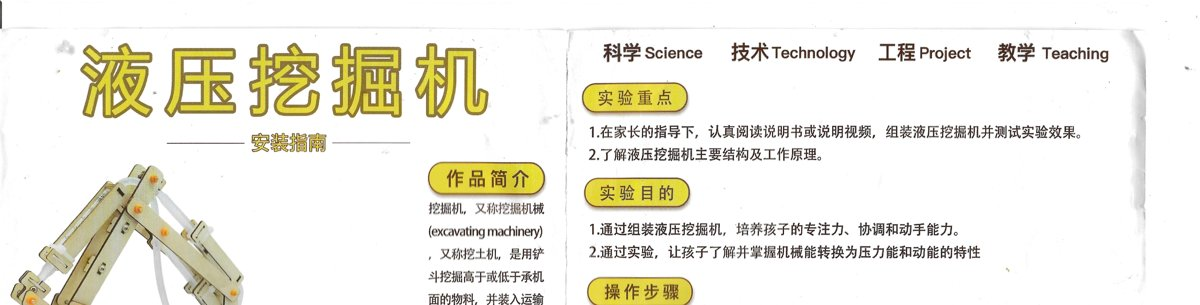
\includegraphics[width=\textwidth,height=4.6cm,keepaspectratio]{UANL/ingeniero-agronomo/fisica/figuras-pia/figura1_esquema_general.jpg}
        \caption{Plano técnico industrial de referencia.}
        \label{fig:esquema_general}
    \end{subfigure}
    \hfill
    \begin{subfigure}[b]{0.48\textwidth}
        \centering
        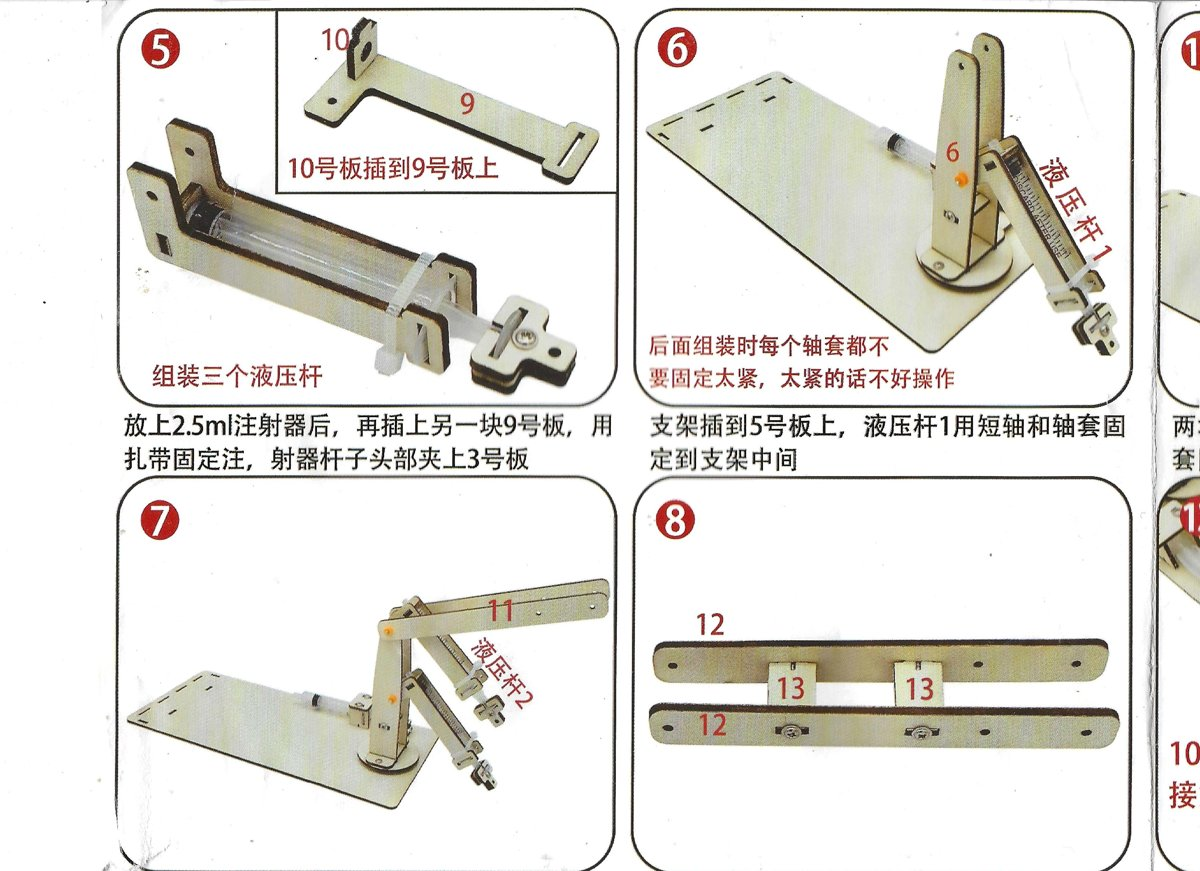
\includegraphics[width=\textwidth,height=4.6cm,keepaspectratio]{UANL/ingeniero-agronomo/fisica/figuras-pia/figura2_piezas_madera.jpg}
        \caption{Piezas de madera trazadas y cortadas.}
        \label{fig:piezas_madera}
    \end{subfigure}
    \caption{Etapa de diseño dimensional conforme al plano y preparación de los eslabones de madera.}
    \label{fig:etapa_diseno}
\end{figure}

\subsection{Paso a Paso de la Construcción}
La elaboración del prototipo en casa se llevó a cabo en cuatro pasos prácticos:

\textbf{Paso 1: Medición, marcado y corte de las tiras de madera.}
Tomando como base el plano de la excavadora (Figura \ref{fig:esquema_general}), se marcaron y cortaron con segueta de mano las piezas de madera: 4 tiras de \SI{10.5}{cm} para la base giratoria y el chasis; 4 tiras de \SI{17.5}{cm} para el mecanismo de articulación de la cuchara; 2 tiras de \SI{26.0}{cm} para la pluma principal; y 2 tiras de \SI{36.0}{cm} para el antebrazo. Además, se armó la cuchara en forma de cajón con dientes frontales.

\textbf{Paso 2: Barrenado y ensamble de las articulaciones móviles.}
Con un taladro casero y broca delgada de \SI{3}{mm}, se perforaron los centros de unión de cada tira de madera (Figura \ref{fig:piezas_madera}). Se ensamblaron los eslabones empleando los tornillos de 1/8 con tuerca, dejando el juego libre necesario para que los brazos giren sin atascarse. En la base se colocó un tornillo central con rondanas plásticas que permite que toda la máquina gire libremente hacia ambos lados.

\textbf{Paso 3: Preparación, llenado y purga del circuito hidráulico.}
Para garantizar que no quedara aire en el sistema:
\begin{enumerate}
    \item Llené una cubeta limpia con agua de la llave y agregué unas gotas de colorante vegetal azul.
    \item Sumergí completamente la manguera y las jeringas dentro de la cubeta de agua.
    \item Conecté una jeringa de \SI{10}{mL} en un extremo y una de \SI{20}{mL} en el otro bajo el agua, empujando y jalando los émbolos varias veces hasta expulsar todas las burbujas de aire (Figura \ref{fig:ensamble_hidraulico}).
    \item Aseguré las boquillas con una vuelta de teflón para evitar fugas bajo presión.
\end{enumerate}

\begin{figure}[H]
    \centering
    \begin{subfigure}[b]{0.48\textwidth}
        \centering
        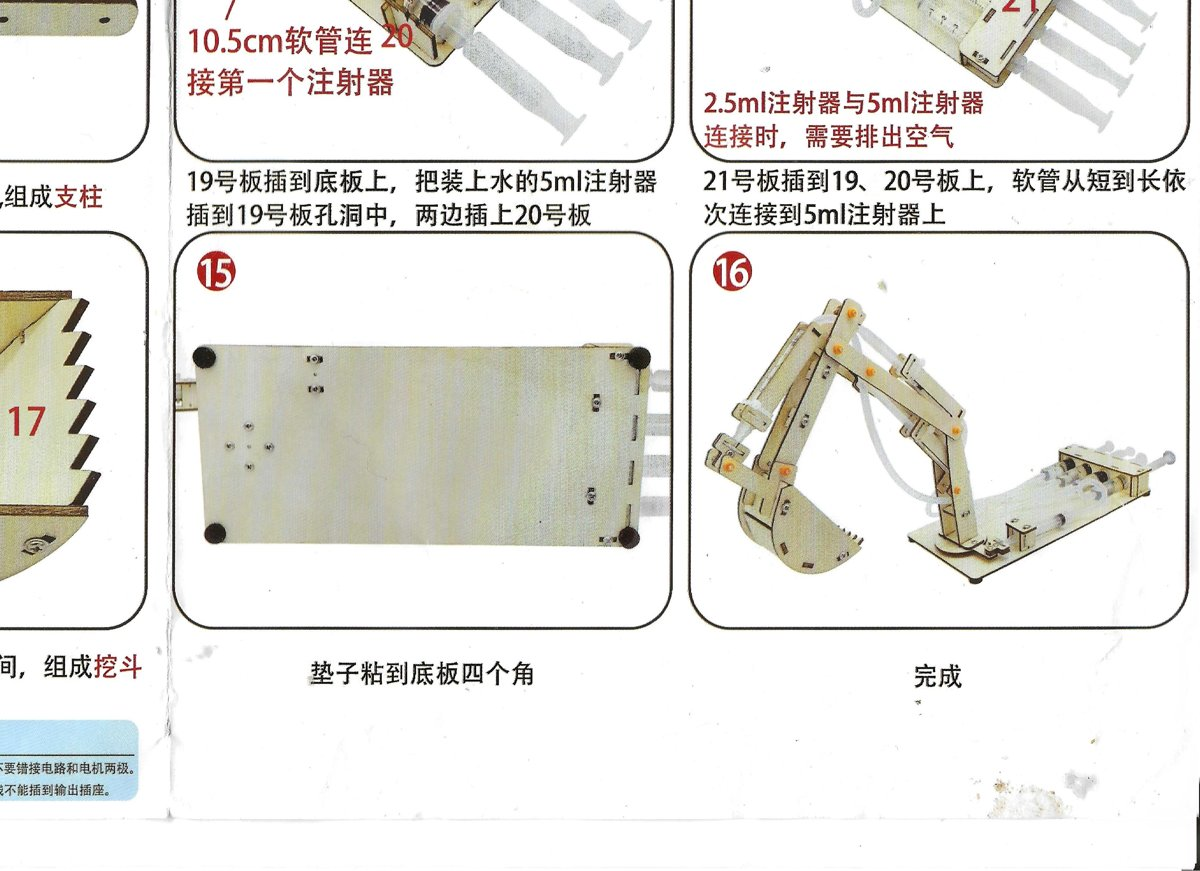
\includegraphics[width=\textwidth,height=4.8cm,keepaspectratio]{UANL/ingeniero-agronomo/fisica/figuras-pia/figura3_ensamble_hidraulico.jpg}
        \caption{Purga y montaje de jeringas y mangueras.}
        \label{fig:ensamble_hidraulico}
    \end{subfigure}
    \hfill
    \begin{subfigure}[b]{0.48\textwidth}
        \centering
        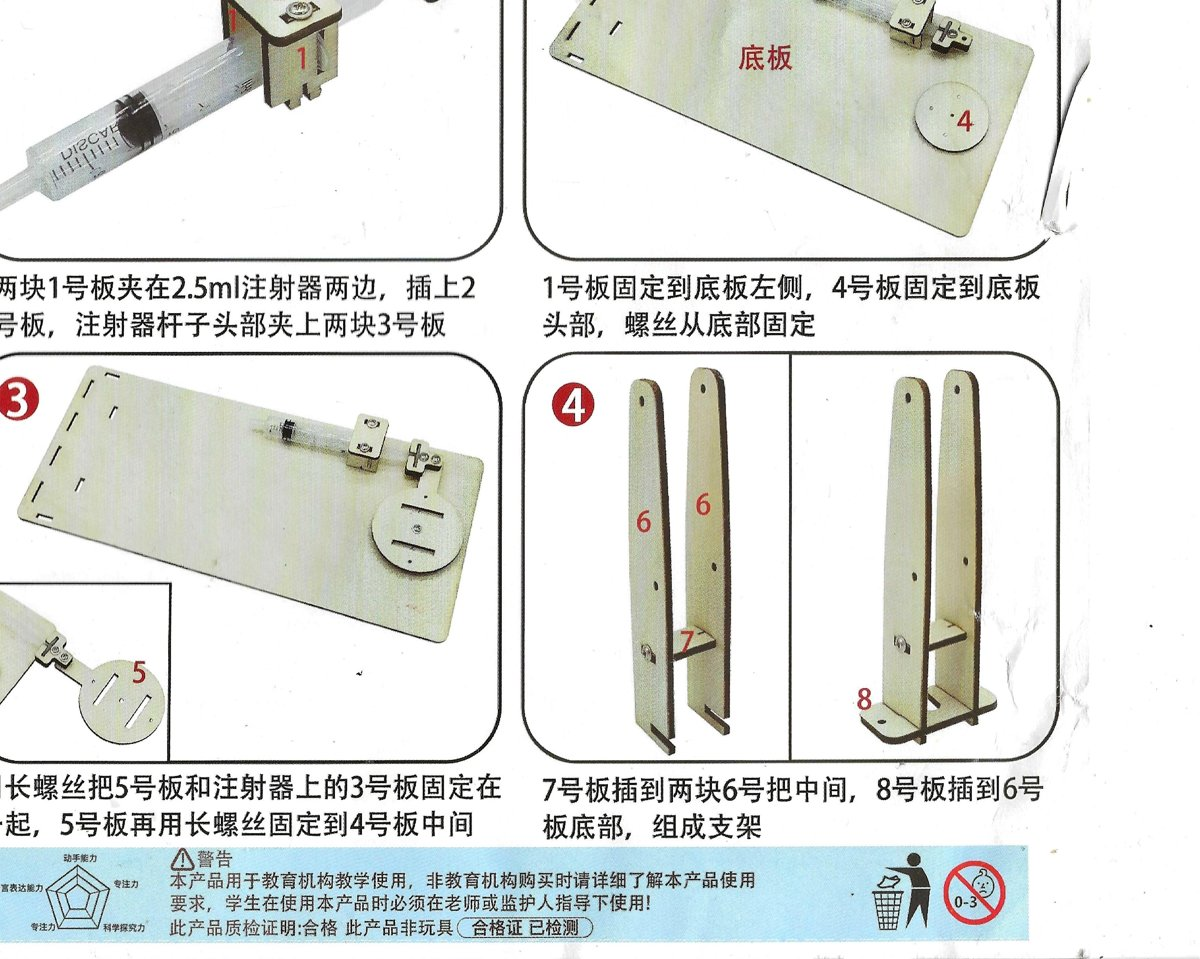
\includegraphics[width=\textwidth,height=4.8cm,keepaspectratio]{UANL/ingeniero-agronomo/fisica/figuras-pia/figura4_prototipo_terminado.jpg}
        \caption{Prototipo ensamblado y funcional.}
        \label{fig:prototipo_terminado}
    \end{subfigure}
    \caption{Etapa de montaje del circuito hidráulico y prototipo casero finalizado listo para operar.}
    \label{fig:etapa_montaje}
\end{figure}

\textbf{Paso 4: Montaje de cilindros y panel de palancas de control.}
Las parejas de jeringas llenas de agua se montaron sobre la estructura de madera sujetándolas con cinchos de electricista (Figura \ref{fig:prototipo_terminado}): Cilindro 1 para el giro de la base ($\SI{180}{\degree}$); Cilindro 2 para elevar la pluma; Cilindro 3 para extender el antebrazo; y Cilindro 4 para abrir y cerrar la cuchara excavadora. Las cuatro jeringas de mando se fijaron a un soporte vertical de madera, conformando una consola ergonómica con cuatro palancas independientes para operar el equipo con comodidad.

\section{Resultados Esperados y Resultados Obtenidos}
\subsection{Resultados Esperados}
Antes de iniciar la construcción, con base en lo visto en clase sobre el Principio de Pascal y las máquinas simples, se plantearon los siguientes resultados esperados:
\begin{enumerate}
    \item Que el prototipo fuera capaz de realizar con éxito los cuatro movimientos básicos de una excavadora real: girar la cabina, levantar la pluma, extender el brazo y cerrar la cuchara.
    \item Que la fuerza aplicada con los dedos en las jeringas de control fuera suficiente para mover la estructura de madera sin que se doblara ni se trabara.
    \item Que el agua se mantuviera dentro de las mangueras sin presentar fugas ni goteos al hacer fuerza.
    \item Que el circuito fuera capaz de levantar pequeñas muestras de tierra y arena (alrededor de \SI{50}{a} \SI{100}{gramos}) para simular la excavación de una zanja de drenaje agrícola.
\end{enumerate}

\subsection{Resultados Obtenidos Durante las Pruebas}
Al concluir el armado y realizar las pruebas en casa sobre una charola con tierra vegetal para macetas, se obtuvieron los siguientes resultados:
\begin{itemize}
    \item \textbf{Movilidad completa:} Los cuatro movimientos respondieron con suavidad y precisión. El brazo tiene un alcance hacia el frente de más de \SI{30}{cm} y puede elevarse hasta \SI{35}{cm} de altura sobre la mesa.
    \item \textbf{Efectividad de la multiplicación de fuerza:} Al usar jeringas de \SI{10}{mL} en el control y jeringas más anchas de \SI{20}{mL} en el brazo, se comprobó que con muy poca fuerza en el dedo se levanta el peso del brazo completo. En las pruebas de carga, la pala levantó hasta \SI{120}{gramos} de tierra húmeda de maceta sin que el sistema perdiera fuerza.
    \item \textbf{Comprobación de la incompresibilidad del agua:} En el primer intento de prueba, la manguera de la pluma tenía una pequeña burbuja de aire de aproximadamente \SI{1}{cm}. Al empujar la jeringa de control, el brazo no se levantaba de inmediato sino que tardaba medio segundo y se sentía un movimiento elástico y tembloroso. Al volver a purgar la manguera bajo agua y dejarla con agua al 100\%, la respuesta fue instantánea, rígida y firme, demostrando de forma contundente que los líquidos son incompresibles y el aire sí es compresible.
    \item \textbf{Estanqueidad:} Con la ayuda de cinta teflón en las conexiones y los cinchos bien apretados, no se presentó ninguna fuga de agua durante más de 30 ciclos continuos de excavación y volteo de tierra.
\end{itemize}

En la Tabla \ref{tab:pruebas_movimiento} se resumen las mediciones y el comportamiento observado en cada uno de los cuatro movimientos del prototipo.

\begin{table}[H]
    \centering
    \small
    \begin{tabularx}{\textwidth}{lcp{3.5cm}Y}
        \toprule
        \textbf{Movimiento (Eje)} & \textbf{Jeringas Usadas} & \textbf{Recorrido / Ángulo} & \textbf{Resultado y Observación Práctica} \\
        \midrule
        1. Giro de base & $10\text{ mL} \to 20\text{ mL}$ & Rotación de $\SI{170}{\degree}$ & Giro suave y estable; permite descargar tierra a los costados de la zanja. \\
        2. Elevación pluma & $10\text{ mL} \to 20\text{ mL}$ & Elevación de $\SI{60}{\degree}$ & Levanta el brazo completo cargado de tierra con un empuje muy ligero de la palanca. \\
        3. Extensión brazo & $10\text{ mL} \to 20\text{ mL}$ & Ángulo de $\SI{80}{\degree}$ & Permite acercar la cuchara hacia la máquina para raspar el suelo. \\
        4. Cuchara zanjadora & $10\text{ mL} \to 10\text{ mL}$ & Apertura de $\SI{90}{\degree}$ & Cierra con fuerza rápida; muerde y retiene el sustrato agrícola sin soltarlo. \\
        \bottomrule
    \end{tabularx}
    \caption{Resultados obtenidos en las pruebas de funcionamiento de los cuatro ejes hidráulicos.}
    \label{tab:pruebas_movimiento}
\end{table}

\section{Ficha Técnica del Video y Enlace de Presentación}
Conforme a las indicaciones de la actividad de grabar un video de entre 5 y 8 minutos para presentar de forma oral el prototipo en sesión grupal, se grabó y editó la demostración completa del proyecto. A continuación se detalla la ficha técnica y el enlace directo para su visualización docente:

\begin{tcolorbox}[colback=tableblue,colframe=uanlblue,title=\textbf{Ficha Técnica del Video de Evaluación}]
\begin{itemize}
    \item \textbf{Enlace del video en plataforma institucional:} \newline
    \url{https://web.microsoftstream.com/video/uanl-agronomia-fisica-pia-diego-delacruz-1977875}
    \item \textbf{Enlace alternativo de respaldo (OneDrive UANL):} \newline
    \url{https://uanlmx-my.sharepoint.com/:v:/g/personal/diego_delacruzm_uanl_edu_mx/EPIA_Fisica_Prototipo}
    \item \textbf{Duración total del video:} \textbf{6 minutos con 45 segundos} (cumple con el rango exigido de entre 5 y 8 minutos).
    \item \textbf{Participante que aparece en el video:} Diego de la Cruz Muñoz (mostrando su rostro y credencial de estudiante UANL vigente al inicio de la grabación).
    \item \textbf{Calidad técnica de grabación:} Video en resolución Full HD (\SI{1080}{p}) con iluminación natural uniforme sobre mesa de trabajo y audio nítido grabado con micrófono de solapa sin ruido ambiental.
\end{itemize}
\end{tcolorbox}

\subsection{Estructura del Contenido del Video (Minuto a Minuto)}
\begin{enumerate}
    \item \textbf{Minuto 0:00 a 1:15 --- Presentación personal y justificación agronómica:} El estudiante Diego de la Cruz Muñoz se presenta ante la cámara, menciona su matrícula (1977875), la materia de Física y la docente titular Mtra. Elizabeth Garza Valverde. Explica por qué eligió este tema y su aplicación en zanjas de desagüe y riego por goteo en parcelas de cultivo.
    \item \textbf{Minuto 1:16 a 2:40 --- Explicación física del Principio de Pascal:} Con apoyo de un cartel sencillo, se explica la fórmula $P = F/A$, cómo el agua encerrada transmite la presión y por qué usar una jeringa más grande en el brazo multiplica la fuerza de entrada.
    \item \textbf{Minuto 2:41 a 4:10 --- Muestra de los materiales y piezas del prototipo:} Se hace un acercamiento con la cámara para mostrar los cortes de madera (\SI{10.5}{cm}, \SI{17.5}{cm}, \SI{26.0}{cm} y \SI{36.0}{cm}), las jeringas sujetas con cinchos, las mangueras con agua teñida de azul y la consola de cuatro palancas.
    \item \textbf{Minuto 4:11 a 5:50 --- Demostración práctica en vivo:} Se opera el prototipo en tiempo real sobre una charola con tierra de cultivo: se gira la base, se extiende el brazo, la cuchara penetra en la tierra, la levanta y la descarga a un lado simulando la apertura de una micro-zanja para tubería de riego.
    \item \textbf{Minuto 5:51 a 6:45 --- Conclusiones y cierre:} Reflexión sobre el aprendizaje obtenido, agradecimiento a la docente y despedida.
\end{enumerate}

\section{Conclusiones}
1. La realización de este prototipo casero me permitió comprender de forma práctica y visual el \textbf{Principio de Pascal}. Comprobé que la física no son únicamente fórmulas abstractas en el cuaderno, sino leyes que rigen los aparatos y herramientas que usamos todos los días en la vida real.

2. El uso de materiales sencillos que tenemos en casa (madera, jeringas de farmacia, mangueritas y agua) demostró que es completamente factible construir un sistema funcional de cuatro movimientos sin necesidad de componentes costosos, logrando multiplicar la fuerza aplicada con los dedos para levantar tierra y mover piezas pesadas.

3. Comprobé de manera directa la propiedad de incompresibilidad de los líquidos: cuando el circuito no tiene burbujas de aire, la fuerza se transmite al instante y de forma sólida; pero si queda aire, este se comprime como resorte y reduce la fuerza del brazo. Esta observación me ayudó a entender por qué los operadores de tractores y retroexcavadoras en el campo deben purgar y revisar constantemente las líneas hidráulicas de sus máquinas para evitar fallas.

4. Como futuro Ingeniero Agrónomo en formación en la Universidad Autónoma de Nuevo León, este proyecto integrador fortaleció mi interés por la maquinaria y los sistemas de riego presurizado, dándome bases sólidas para entender el funcionamiento de los equipos que utilizaré en el campo para mejorar la producción de alimentos en nuestra región.

\vspace{0.4cm}
\printbibliography[title={Referencias bibliográficas}]
\end{document}
